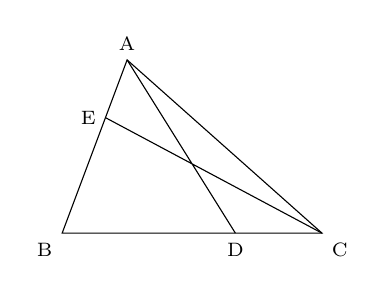
\begin{tikzpicture}[scale=0.55]
\coordinate (B) at (0,0); \coordinate (C) at (6,0); \coordinate (A) at (1.5,4);
\coordinate (D) at (4,0); \coordinate (E) at (1,2.667);
\draw (A)--(B)--(C)--cycle; \draw (A)--(D) (C)--(E);
\node[above] at (A){\scriptsize A}; \node[below left] at (B){\scriptsize B}; \node[below right] at (C){\scriptsize C};
\node[below] at (D){\scriptsize D}; \node[left] at (E){\scriptsize E};
\end{tikzpicture}